\documentclass{article}

\usepackage{graphicx}
\usepackage{booktabs} 

\begin{document}

\section{Didge Report No 0}

\subsection{General information}
\begin{centering}

\begin{figure}[!htb]
\center{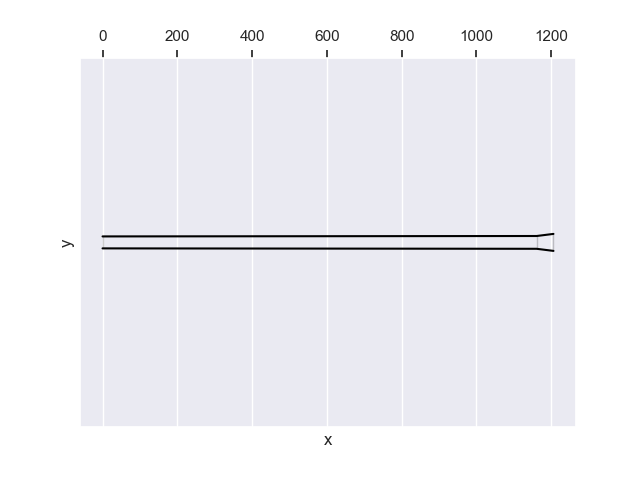
\includegraphics[width=\textwidth]
{0_didge.png}}
\end{figure}
\begin{tabular}{lr}
\toprule
         length & 1206.116798 \\
      bell size &   45.456819 \\
number segments &    3.000000 \\
\bottomrule
\end{tabular}
\end{centering}
\subsection{Tuning}
\begin{centering}
\begin{tabular}{rrrrrl}
\toprule
 freq &    impedance &  rel\_imp &  note-number &  cent-diff & note-name \\
\midrule
 73.0 & 2.863653e+07 & 1.000000 &          -31 &   9.842186 &        D1 \\
 73.0 & 2.863653e+07 & 1.000000 &          -31 &   9.842186 &        D1 \\
215.0 & 1.202496e+07 & 0.419917 &          -12 &  39.800237 &        A3 \\
357.0 & 6.607961e+06 & 0.230753 &           -4 & -38.104661 &        F3 \\
501.0 & 4.073509e+06 & 0.142249 &            2 & -24.768496 &        B4 \\
\bottomrule
\end{tabular}
\end{centering}
\begin{centering}
\subsection{Sound Spektra}

\begin{figure}[!htb]
\center{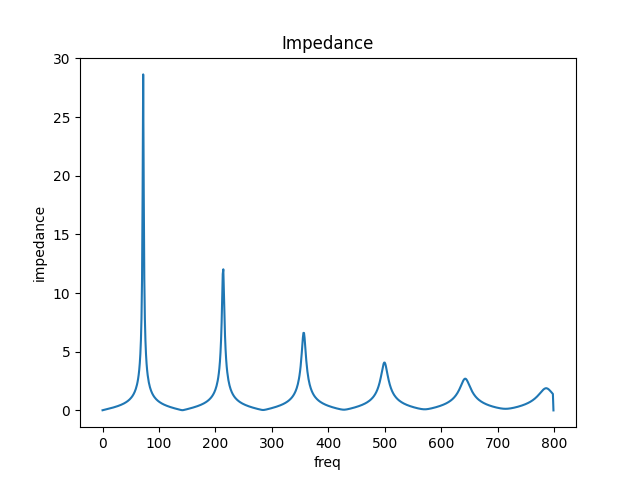
\includegraphics[width=\textwidth]
{0_impedance.png}}
\end{figure}

\begin{figure}[!htb]
\center{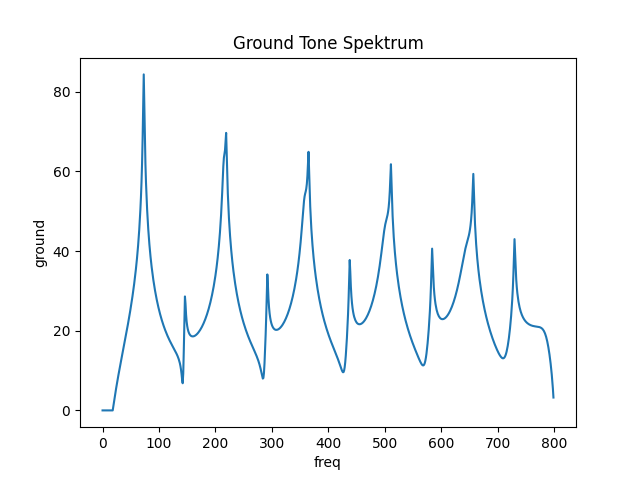
\includegraphics[width=\textwidth]
{0_ground.png}}
\end{figure}

\begin{figure}[!htb]
\center{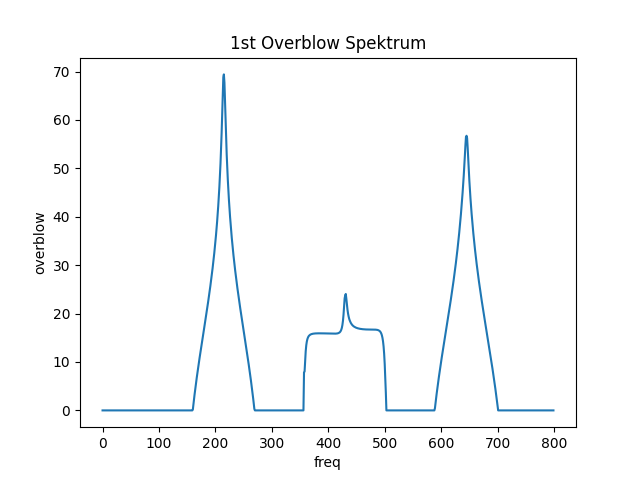
\includegraphics[width=\textwidth]
{0_overblow.png}}
\end{figure}
\end{centering}
\section{Didge Report No 1}

\subsection{General information}
\begin{centering}

\begin{figure}[!htb]
\center{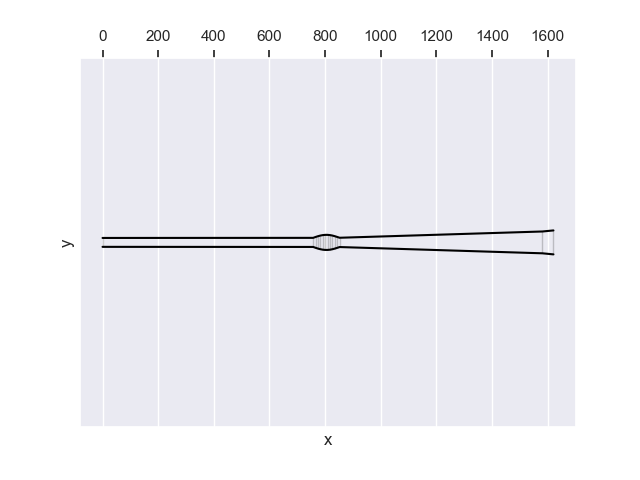
\includegraphics[width=\textwidth]
{1_didge.png}}
\end{figure}
\begin{tabular}{lr}
\toprule
         length & 1620.623613 \\
      bell size &   86.086643 \\
number segments &   15.000000 \\
\bottomrule
\end{tabular}
\end{centering}
\subsection{Tuning}
\begin{centering}
\begin{tabular}{rrrrrl}
\toprule
 freq &    impedance &  rel\_imp &  note-number &  cent-diff & note-name \\
\midrule
 72.8 & 3.089921e+07 & 1.000000 &          -31 &  14.591802 &        D1 \\
166.0 & 7.499440e+06 & 0.242707 &          -17 & -12.415661 &        E2 \\
264.0 & 3.252943e+06 & 0.105276 &           -9 & -15.641287 &        C3 \\
369.0 & 4.475765e+06 & 0.144850 &           -3 &   4.659249 &       F\#3 \\
580.0 & 3.254196e+06 & 0.105316 &            5 &  21.740748 &        D4 \\
\bottomrule
\end{tabular}
\end{centering}
\begin{centering}
\subsection{Sound Spektra}

\begin{figure}[!htb]
\center{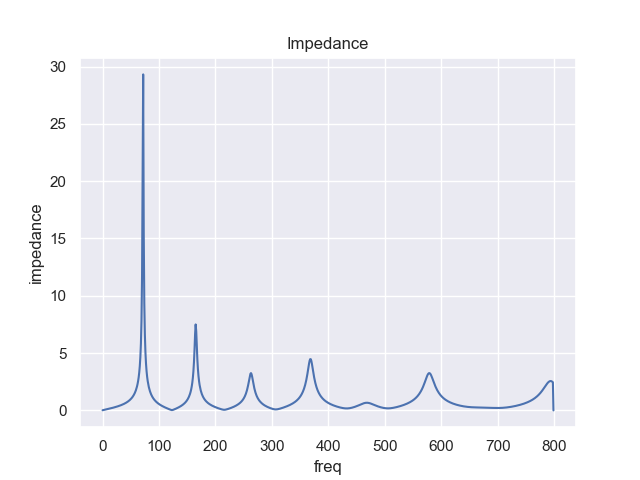
\includegraphics[width=\textwidth]
{1_impedance.png}}
\end{figure}

\begin{figure}[!htb]
\center{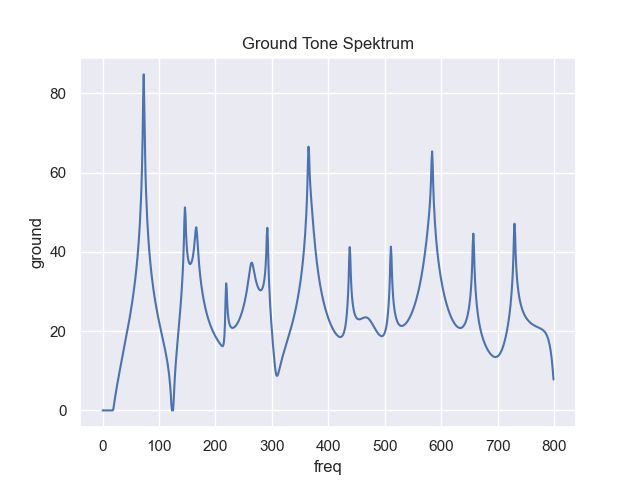
\includegraphics[width=\textwidth]
{1_ground.png}}
\end{figure}

\begin{figure}[!htb]
\center{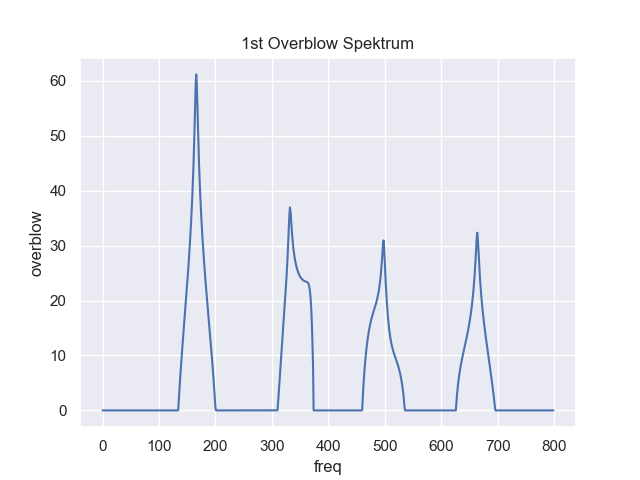
\includegraphics[width=\textwidth]
{1_overblow.png}}
\end{figure}
\end{centering}
\section{Didge Report No 2}

\subsection{General information}
\begin{centering}

\begin{figure}[!htb]
\center{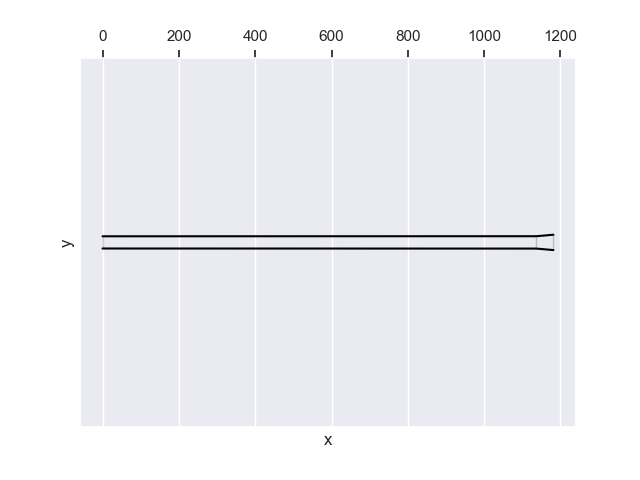
\includegraphics[width=\textwidth]
{2_didge.png}}
\end{figure}
\begin{tabular}{lr}
\toprule
         length & 1181.563291 \\
      bell size &   40.277813 \\
number segments &    3.000000 \\
\bottomrule
\end{tabular}
\end{centering}
\subsection{Tuning}
\begin{centering}
\begin{tabular}{rrrrrl}
\toprule
 freq &    impedance &  rel\_imp &  note-number &  cent-diff & note-name \\
\midrule
 72.7 & 2.966377e+07 & 1.000000 &          -31 &  16.971505 &        D1 \\
218.0 & 1.290594e+07 & 0.435074 &          -12 &  15.810466 &        A3 \\
364.0 & 7.370868e+06 & 0.248480 &           -3 &  28.278088 &       F\#3 \\
510.0 & 4.659704e+06 & 0.157084 &            3 &  44.407532 &        C4 \\
656.0 & 3.153374e+06 & 0.106304 &            7 &   8.569251 &        E4 \\
\bottomrule
\end{tabular}
\end{centering}
\begin{centering}
\subsection{Sound Spektra}

\begin{figure}[!htb]
\center{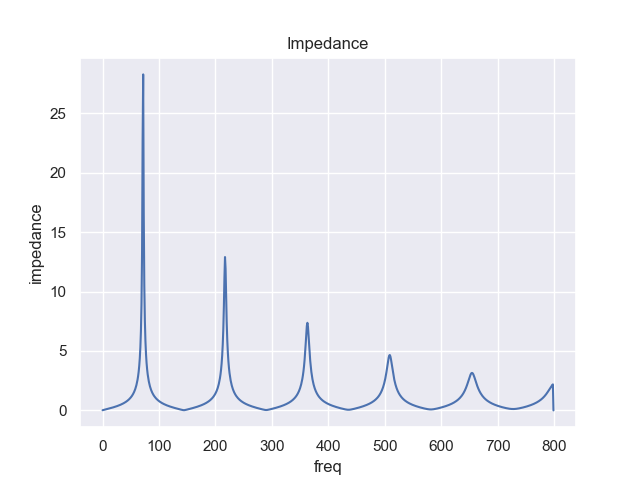
\includegraphics[width=\textwidth]
{2_impedance.png}}
\end{figure}

\begin{figure}[!htb]
\center{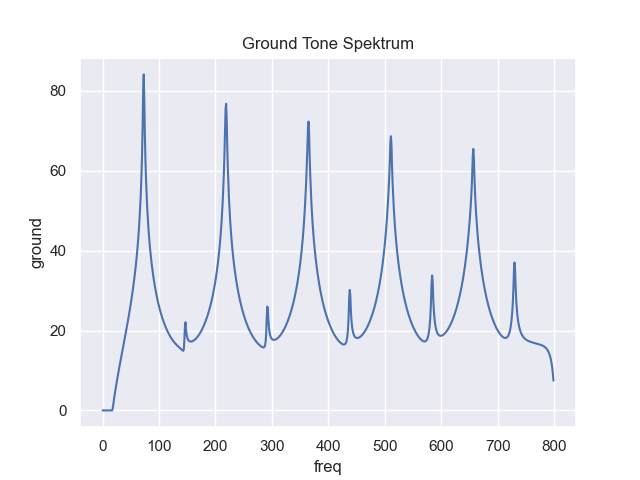
\includegraphics[width=\textwidth]
{2_ground.png}}
\end{figure}

\begin{figure}[!htb]
\center{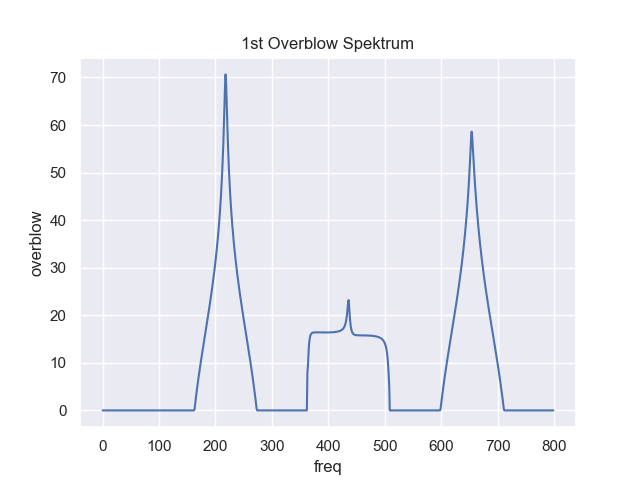
\includegraphics[width=\textwidth]
{2_overblow.png}}
\end{figure}
\end{centering}
\section{Didge Report No 3}

\subsection{General information}
\begin{centering}

\begin{figure}[!htb]
\center{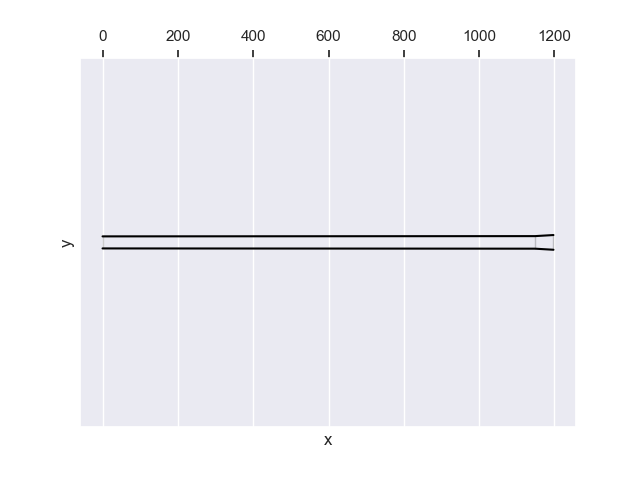
\includegraphics[width=\textwidth]
{3_didge.png}}
\end{figure}
\begin{tabular}{lr}
\toprule
         length & 1197.324180 \\
      bell size &   39.087808 \\
number segments &    3.000000 \\
\bottomrule
\end{tabular}
\end{centering}
\subsection{Tuning}
\begin{centering}
\begin{tabular}{rrrrrl}
\toprule
 freq &    impedance &  rel\_imp &  note-number &  cent-diff & note-name \\
\midrule
 72.6 & 2.944907e+07 & 1.000000 &          -31 &  19.354484 &        D1 \\
215.0 & 1.316961e+07 & 0.447199 &          -12 &  39.800237 &        A3 \\
359.0 & 7.705165e+06 & 0.261644 &           -4 & -47.776384 &        F3 \\
502.0 & 4.918149e+06 & 0.167005 &            2 & -28.220609 &        B4 \\
646.0 & 3.375525e+06 & 0.114622 &            7 &  35.163231 &        E4 \\
\bottomrule
\end{tabular}
\end{centering}
\begin{centering}
\subsection{Sound Spektra}

\begin{figure}[!htb]
\center{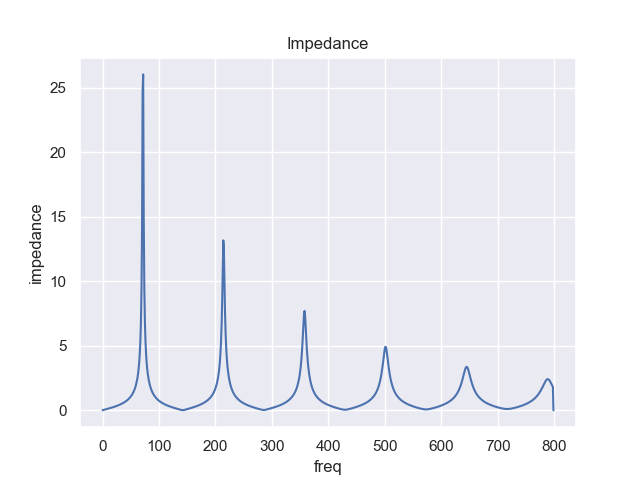
\includegraphics[width=\textwidth]
{3_impedance.png}}
\end{figure}

\begin{figure}[!htb]
\center{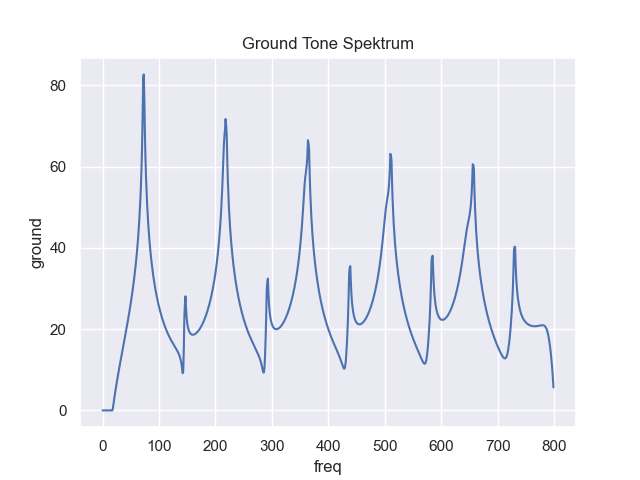
\includegraphics[width=\textwidth]
{3_ground.png}}
\end{figure}

\begin{figure}[!htb]
\center{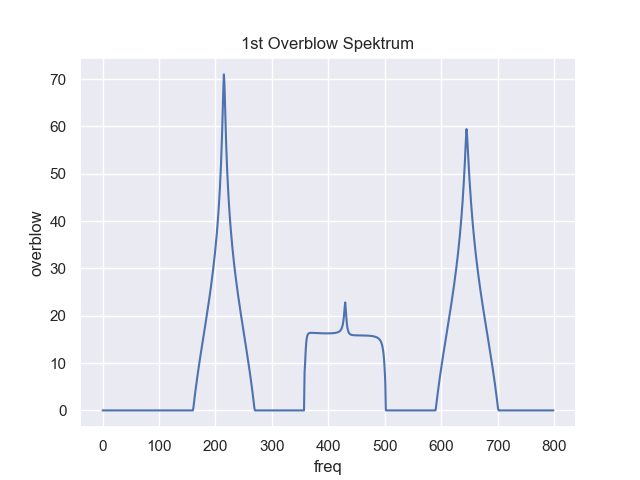
\includegraphics[width=\textwidth]
{3_overblow.png}}
\end{figure}
\end{centering}
\section{Didge Report No 4}

\subsection{General information}
\begin{centering}

\begin{figure}[!htb]
\center{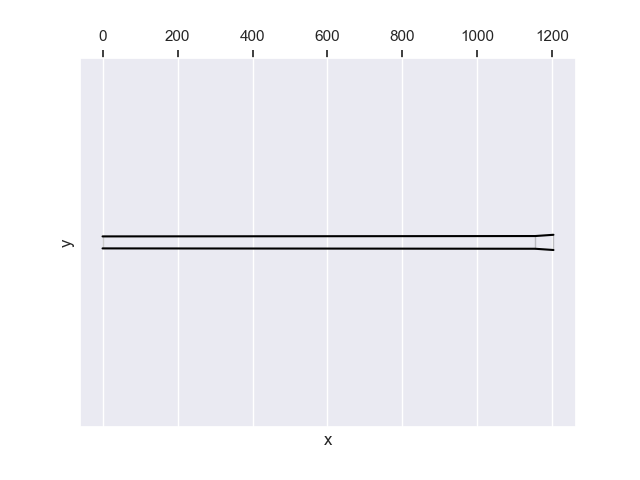
\includegraphics[width=\textwidth]
{4_didge.png}}
\end{figure}
\begin{tabular}{lr}
\toprule
         length & 1202.702944 \\
      bell size &   40.614292 \\
number segments &    3.000000 \\
\bottomrule
\end{tabular}
\end{centering}
\subsection{Tuning}
\begin{centering}
\begin{tabular}{rrrrrl}
\toprule
 freq &    impedance &  rel\_imp &  note-number &  cent-diff & note-name \\
\midrule
 72.8 & 2.921257e+07 & 1.000000 &          -31 &  14.591802 &        D1 \\
215.0 & 1.289333e+07 & 0.441363 &          -12 &  39.800237 &        A3 \\
358.0 & 7.420614e+06 & 0.254021 &           -4 & -42.947276 &        F3 \\
501.0 & 4.727245e+06 & 0.161822 &            2 & -24.768496 &        B4 \\
644.0 & 3.208371e+06 & 0.109828 &            7 &  40.531402 &        E4 \\
\bottomrule
\end{tabular}
\end{centering}
\begin{centering}
\subsection{Sound Spektra}

\begin{figure}[!htb]
\center{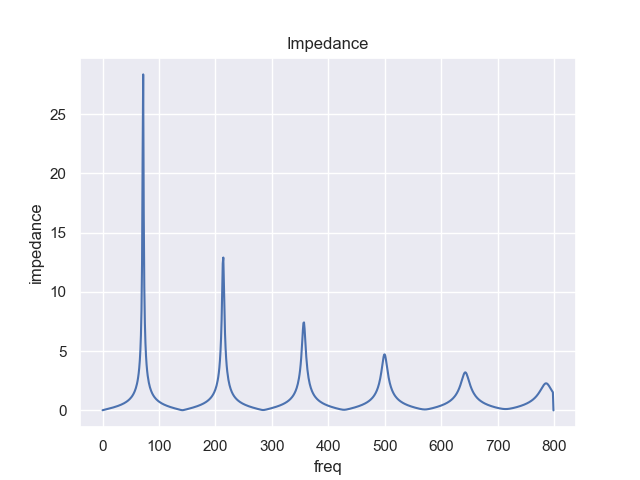
\includegraphics[width=\textwidth]
{4_impedance.png}}
\end{figure}

\begin{figure}[!htb]
\center{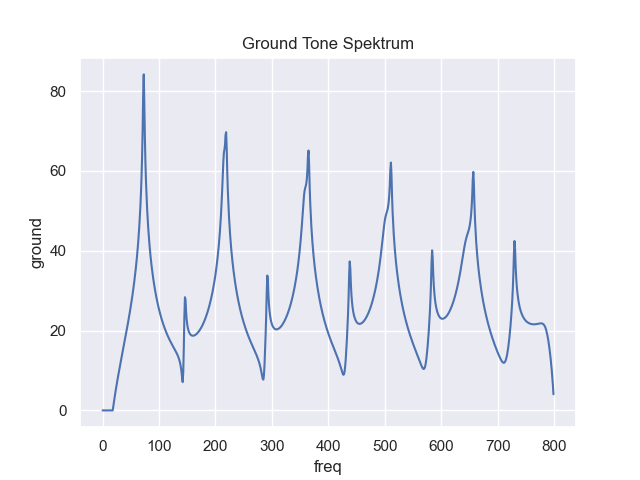
\includegraphics[width=\textwidth]
{4_ground.png}}
\end{figure}

\begin{figure}[!htb]
\center{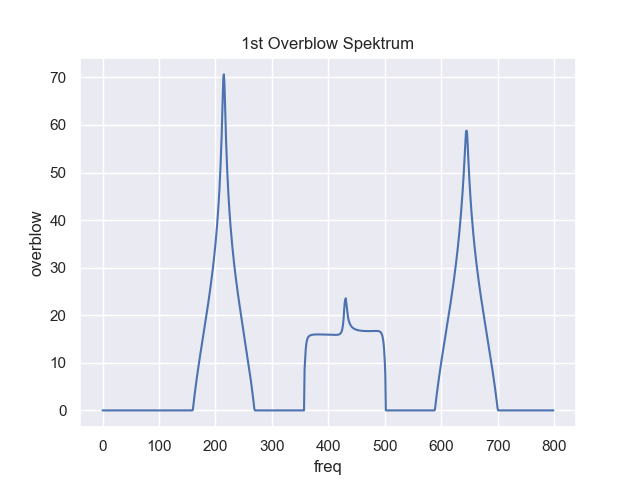
\includegraphics[width=\textwidth]
{4_overblow.png}}
\end{figure}
\end{centering}
\section{Didge Report No 5}

\subsection{General information}
\begin{centering}

\begin{figure}[!htb]
\center{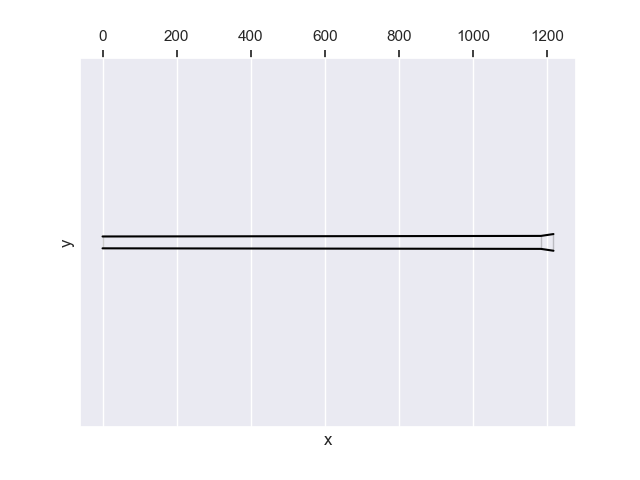
\includegraphics[width=\textwidth]
{5_didge.png}}
\end{figure}
\begin{tabular}{lr}
\toprule
         length & 1217.149743 \\
      bell size &   44.997280 \\
number segments &    3.000000 \\
\bottomrule
\end{tabular}
\end{centering}
\subsection{Tuning}
\begin{centering}
\begin{tabular}{rrrrrl}
\toprule
 freq &    impedance &  rel\_imp &  note-number &  cent-diff & note-name \\
\midrule
 72.8 & 2.842620e+07 & 1.000000 &          -31 &  14.591802 &        D1 \\
212.0 & 1.224135e+07 & 0.430636 &          -13 & -35.872889 &       G\#2 \\
353.0 & 6.836040e+06 & 0.240484 &           -4 & -18.597592 &        F3 \\
495.0 & 4.271988e+06 & 0.150283 &            2 &  -3.910002 &        B4 \\
636.0 & 2.874656e+06 & 0.101127 &            6 & -37.827890 &       D\#4 \\
\bottomrule
\end{tabular}
\end{centering}
\begin{centering}
\subsection{Sound Spektra}

\begin{figure}[!htb]
\center{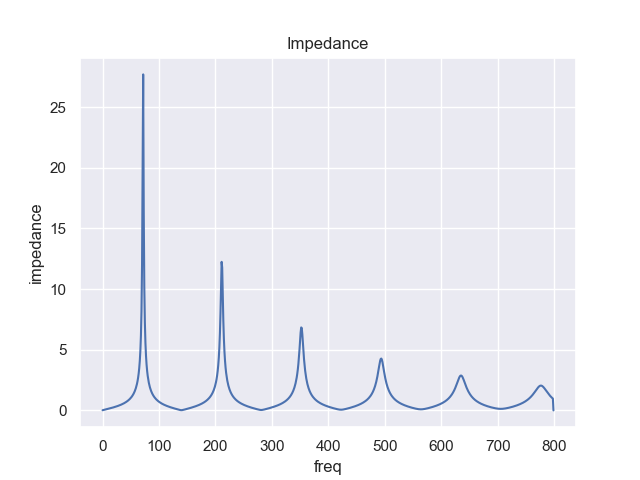
\includegraphics[width=\textwidth]
{5_impedance.png}}
\end{figure}

\begin{figure}[!htb]
\center{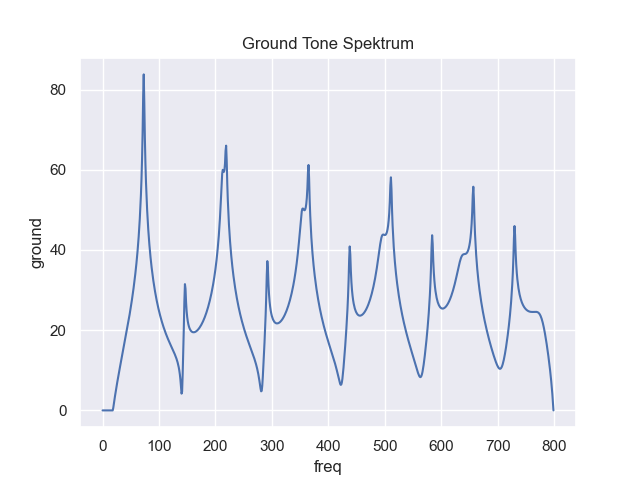
\includegraphics[width=\textwidth]
{5_ground.png}}
\end{figure}

\begin{figure}[!htb]
\center{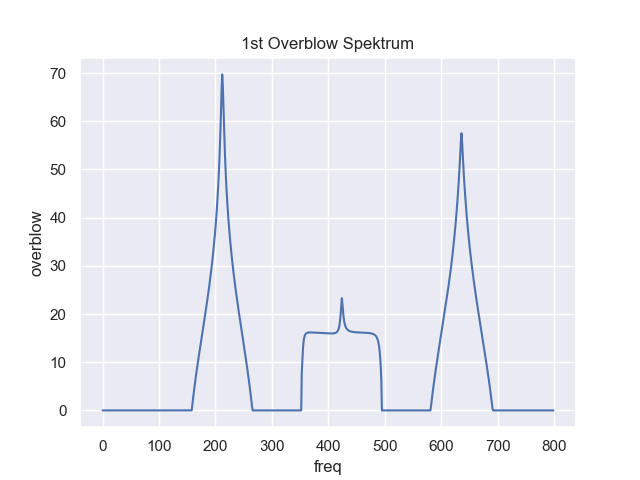
\includegraphics[width=\textwidth]
{5_overblow.png}}
\end{figure}
\end{centering}
\section{Didge Report No 6}

\subsection{General information}
\begin{centering}

\begin{figure}[!htb]
\center{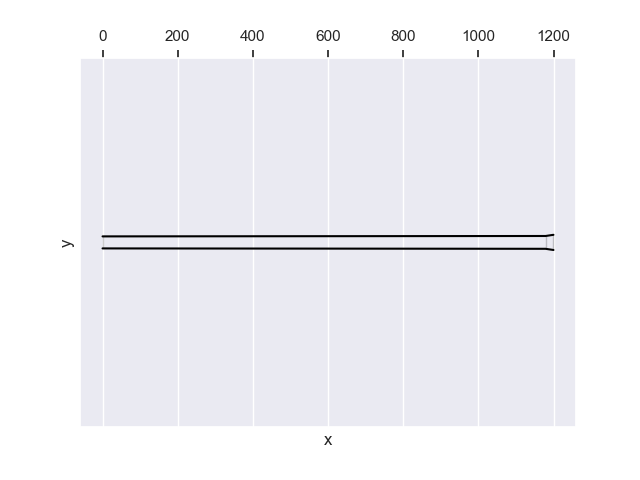
\includegraphics[width=\textwidth]
{6_didge.png}}
\end{figure}
\begin{tabular}{lr}
\toprule
         length & 1199.815921 \\
      bell size &   40.391546 \\
number segments &    3.000000 \\
\bottomrule
\end{tabular}
\end{centering}
\subsection{Tuning}
\begin{centering}
\begin{tabular}{rrrrrl}
\toprule
 freq &    impedance &  rel\_imp &  note-number &  cent-diff & note-name \\
\midrule
 72.8 & 2.914192e+07 & 1.000000 &          -31 &  14.591802 &        D1 \\
214.0 & 1.285693e+07 & 0.441183 &          -12 &  47.871273 &        A3 \\
357.0 & 7.579598e+06 & 0.260093 &           -4 & -38.104661 &        F3 \\
500.0 & 4.872268e+06 & 0.167191 &            2 & -21.309485 &        B4 \\
643.0 & 3.360636e+06 & 0.115320 &            7 &  43.221743 &        E4 \\
\bottomrule
\end{tabular}
\end{centering}
\begin{centering}
\subsection{Sound Spektra}

\begin{figure}[!htb]
\center{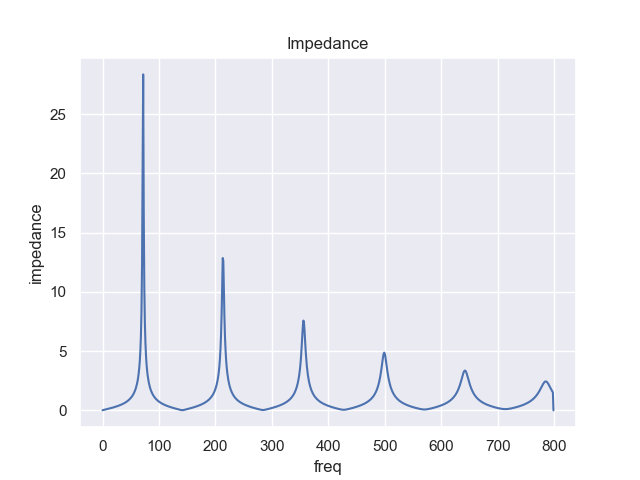
\includegraphics[width=\textwidth]
{6_impedance.png}}
\end{figure}

\begin{figure}[!htb]
\center{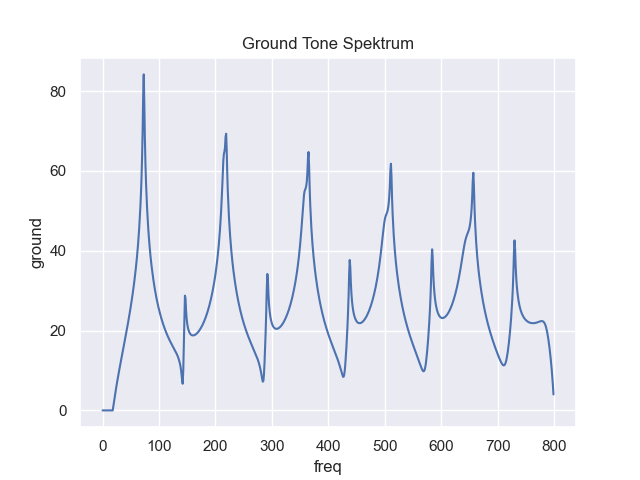
\includegraphics[width=\textwidth]
{6_ground.png}}
\end{figure}

\begin{figure}[!htb]
\center{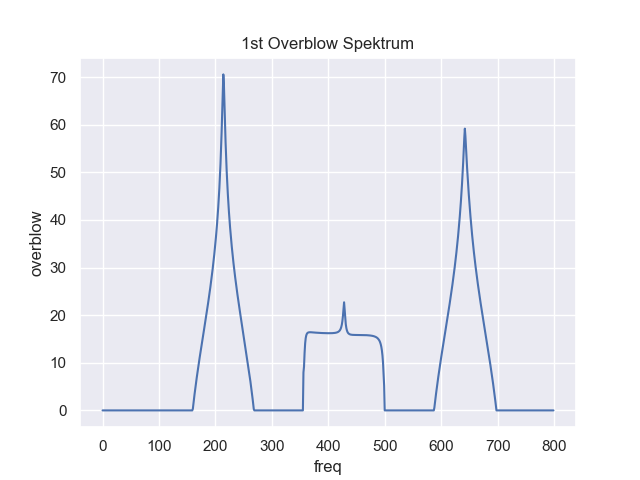
\includegraphics[width=\textwidth]
{6_overblow.png}}
\end{figure}
\end{centering}
\section{Didge Report No 7}

\subsection{General information}
\begin{centering}

\begin{figure}[!htb]
\center{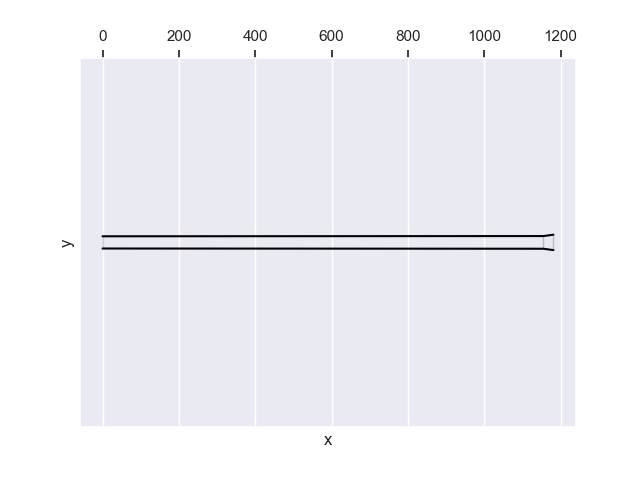
\includegraphics[width=\textwidth]
{7_didge.png}}
\end{figure}
\begin{tabular}{lr}
\toprule
         length & 1181.241718 \\
      bell size &   40.458471 \\
number segments &    3.000000 \\
\bottomrule
\end{tabular}
\end{centering}
\subsection{Tuning}
\begin{centering}
\begin{tabular}{rrrrrl}
\toprule
 freq &    impedance &  rel\_imp &  note-number &  cent-diff & note-name \\
\midrule
 73.3 & 2.939718e+07 & 1.000000 &          -31 &   2.742104 &        D1 \\
218.0 & 1.292811e+07 & 0.439774 &          -12 &  15.810466 &        A3 \\
363.0 & 7.436384e+06 & 0.252962 &           -3 &  33.040771 &       F\#3 \\
508.0 & 4.725644e+06 & 0.160752 &            2 & -48.789968 &        B4 \\
654.0 & 3.253057e+06 & 0.110659 &            7 &  13.855466 &        E4 \\
\bottomrule
\end{tabular}
\end{centering}
\begin{centering}
\subsection{Sound Spektra}

\begin{figure}[!htb]
\center{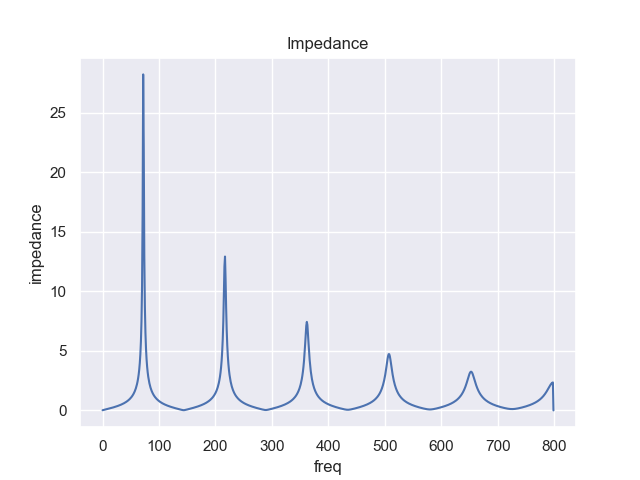
\includegraphics[width=\textwidth]
{7_impedance.png}}
\end{figure}

\begin{figure}[!htb]
\center{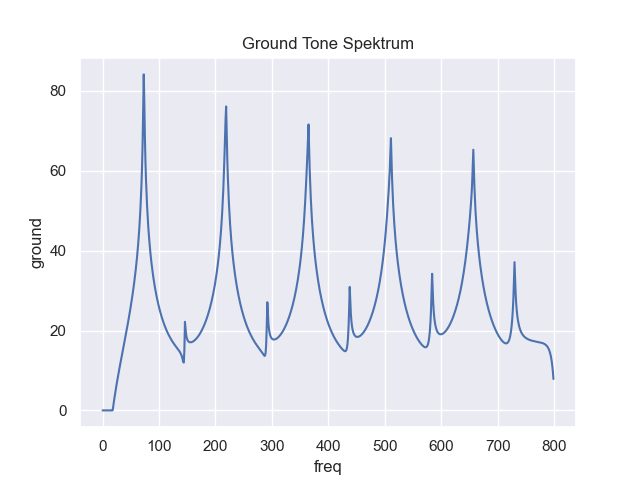
\includegraphics[width=\textwidth]
{7_ground.png}}
\end{figure}

\begin{figure}[!htb]
\center{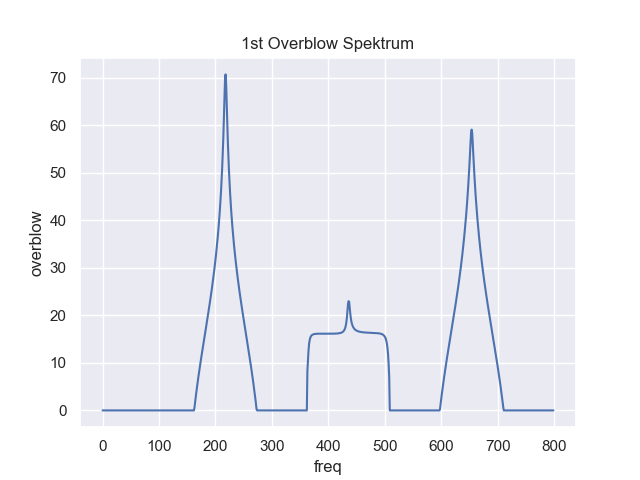
\includegraphics[width=\textwidth]
{7_overblow.png}}
\end{figure}
\end{centering}
\section{Didge Report No 8}

\subsection{General information}
\begin{centering}

\begin{figure}[!htb]
\center{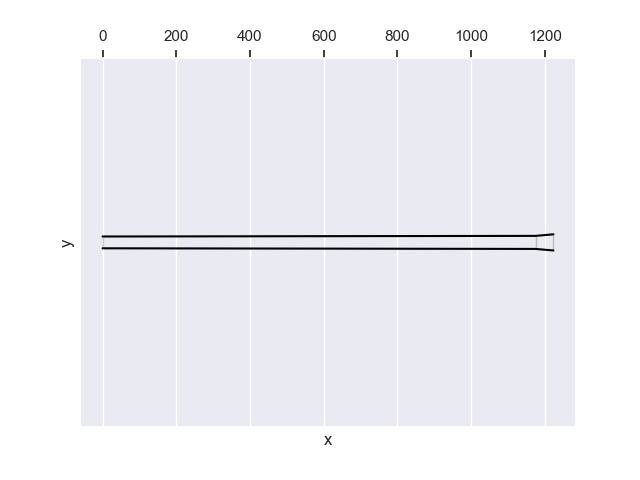
\includegraphics[width=\textwidth]
{8_didge.png}}
\end{figure}
\begin{tabular}{lr}
\toprule
         length & 1223.217255 \\
      bell size &   43.868373 \\
number segments &    3.000000 \\
\bottomrule
\end{tabular}
\end{centering}
\subsection{Tuning}
\begin{centering}
\begin{tabular}{rrrrrl}
\toprule
 freq &    impedance &  rel\_imp &  note-number &  cent-diff & note-name \\
\midrule
 72.9 & 2.848212e+07 & 1.000000 &          -31 &  12.215365 &        D1 \\
212.0 & 1.252820e+07 & 0.439862 &          -13 & -35.872889 &       G\#2 \\
352.0 & 7.047901e+06 & 0.247450 &           -4 & -13.686286 &        F3 \\
493.0 & 4.387339e+06 & 0.154038 &            2 &   3.099053 &        B4 \\
634.0 & 2.930503e+06 & 0.102889 &            6 & -32.375180 &       D\#4 \\
\bottomrule
\end{tabular}
\end{centering}
\begin{centering}
\subsection{Sound Spektra}

\begin{figure}[!htb]
\center{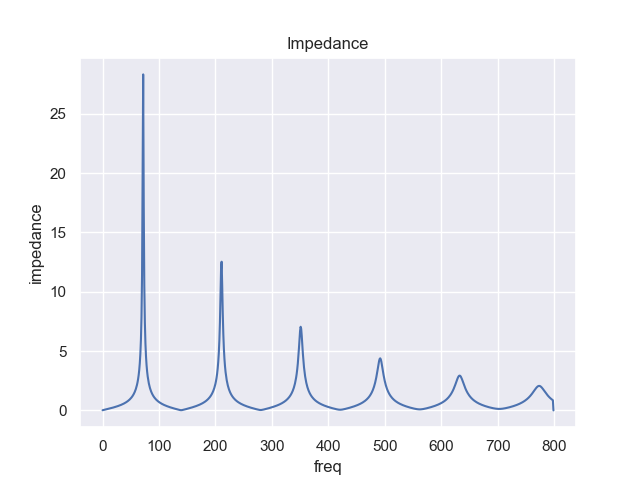
\includegraphics[width=\textwidth]
{8_impedance.png}}
\end{figure}

\begin{figure}[!htb]
\center{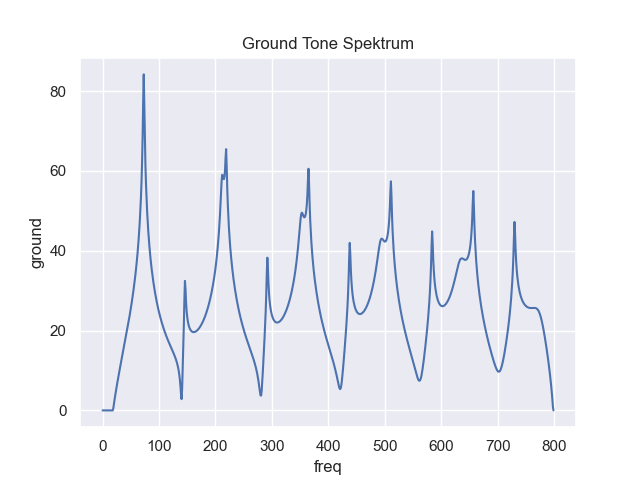
\includegraphics[width=\textwidth]
{8_ground.png}}
\end{figure}

\begin{figure}[!htb]
\center{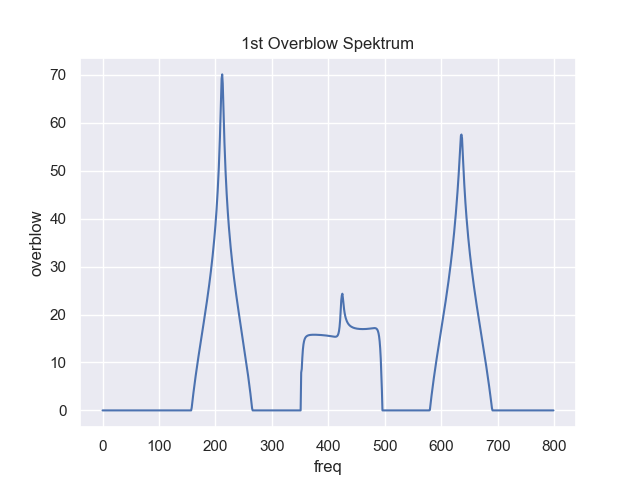
\includegraphics[width=\textwidth]
{8_overblow.png}}
\end{figure}
\end{centering}
\section{Didge Report No 9}

\subsection{General information}
\begin{centering}

\begin{figure}[!htb]
\center{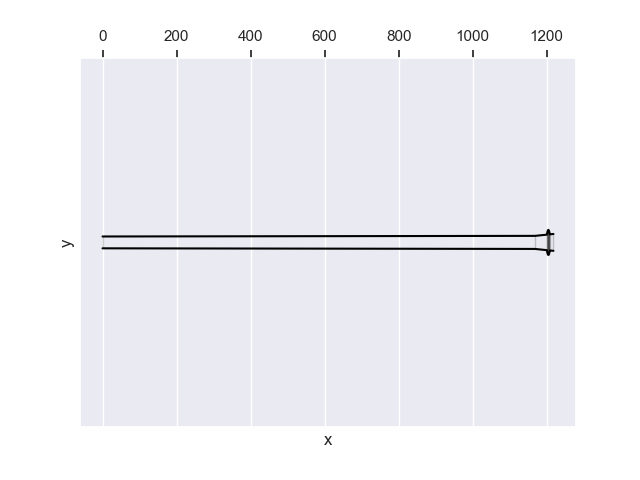
\includegraphics[width=\textwidth]
{9_didge.png}}
\end{figure}
\begin{tabular}{lr}
\toprule
         length & 1218.158455 \\
      bell size &   45.497965 \\
number segments &   15.000000 \\
\bottomrule
\end{tabular}
\end{centering}
\subsection{Tuning}
\begin{centering}
\begin{tabular}{rrrrrl}
\toprule
 freq &    impedance &  rel\_imp &  note-number &  cent-diff & note-name \\
\midrule
 72.9 & 2.933833e+07 & 1.000000 &          -31 &  12.215365 &        D1 \\
212.0 & 1.394286e+07 & 0.475244 &          -13 & -35.872889 &       G\#2 \\
352.0 & 8.015424e+06 & 0.273207 &           -4 & -13.686286 &        F3 \\
493.0 & 5.043319e+06 & 0.171902 &            2 &   3.099053 &        B4 \\
634.0 & 3.263693e+06 & 0.111243 &            6 & -32.375180 &       D\#4 \\
\bottomrule
\end{tabular}
\end{centering}
\begin{centering}
\subsection{Sound Spektra}

\begin{figure}[!htb]
\center{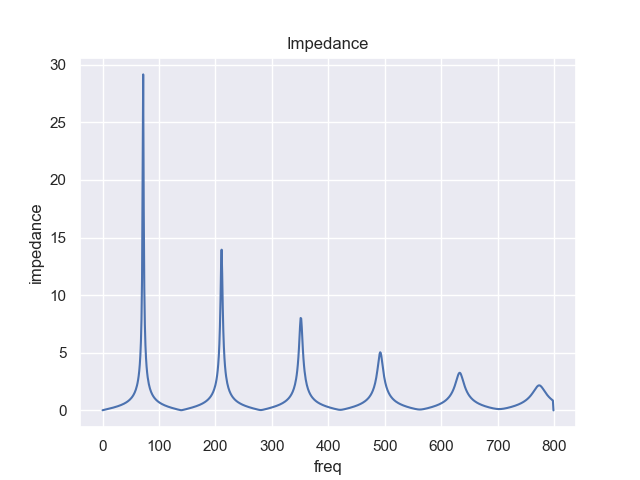
\includegraphics[width=\textwidth]
{9_impedance.png}}
\end{figure}

\begin{figure}[!htb]
\center{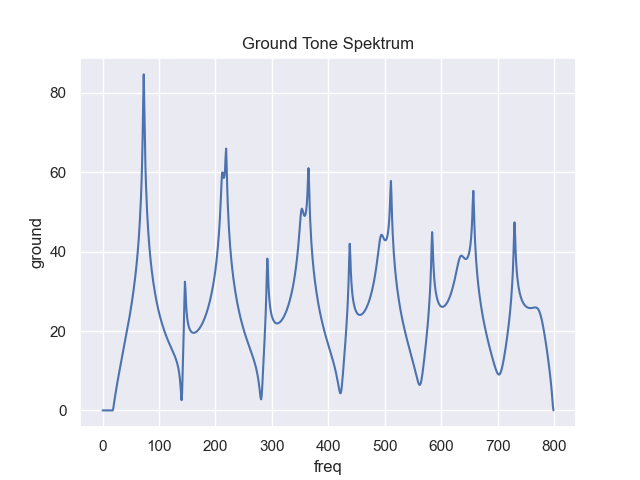
\includegraphics[width=\textwidth]
{9_ground.png}}
\end{figure}

\begin{figure}[!htb]
\center{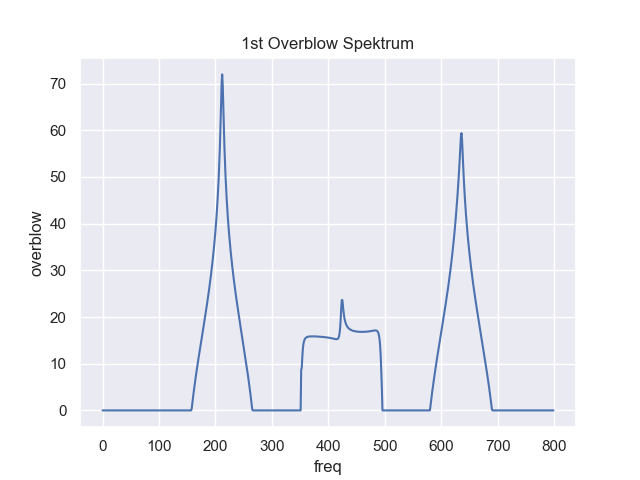
\includegraphics[width=\textwidth]
{9_overblow.png}}
\end{figure}
\end{centering}
\end{document}